\documentclass[11pt,border=5pt]{standalone}
\usepackage{fontspec}
\setmainfont{cmunrm.otf}[BoldFont=cmunbx.otf,ItalicFont=cmunti.otf,BoldItalicFont=cmunbi.otf]
\usepackage{amsmath}
\usepackage{unicode-math}
\setmathfont{NewCMMath-Regular.otf}
\usepackage{tikz}
\usetikzlibrary{arrows.meta,patterns,angles,quotes}
\begin{document}
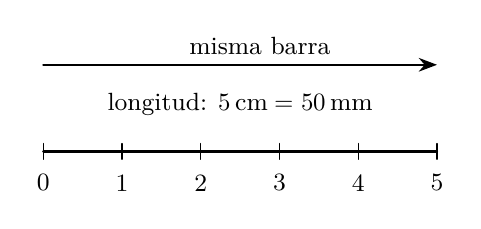
\begin{tikzpicture}[>=Stealth,font=\small,line cap=round,line join=round]
\draw[thick] (0,0) -- (5,0);
\draw[] (0,-0.1) -- (0,0.1);
\node at (0,-0.4) {0};
\draw[] (1,-0.1) -- (1,0.1);
\node at (1,-0.4) {1};
\draw[] (2,-0.1) -- (2,0.1);
\node at (2,-0.4) {2};
\draw[] (3,-0.1) -- (3,0.1);
\node at (3,-0.4) {3};
\draw[] (4,-0.1) -- (4,0.1);
\node at (4,-0.4) {4};
\draw[] (5,-0.1) -- (5,0.1);
\node at (5,-0.4) {5};
\node at (2.5,0.6) {longitud: $5\,\mathrm{cm}=50\,\mathrm{mm}$};
\draw[->,thick] (0,1.1) -- (5,1.1) node[pos=0.55,above] {misma barra};

\end{tikzpicture}
\end{document}
